% !TEX root = Thesis.tex
\documentclass[grad]{uoit-thesis}

% !TEX root = Thesis.tex
\usepackage{morewrites}									% Greedy packages...
\usepackage{fontspec}									% Use nicer system fonts
%\usepackage{mathdesign}
\usepackage{graphicx}									% Pretty pictures
\usepackage{todo}										% List of things to do
\usepackage{amsmath}									% Allow use of amsthm
\usepackage{amsthm}										% Pretty theorem environments
\usepackage{amssymb}									% More math symbols
\usepackage{algorithm}									% Pretty algorithm environment
\usepackage{algorithmic}								% Pretty algorithms
\usepackage[nounderscore]{syntax}						% BNF grammars
\usepackage{minted}										% Pretty code
\usepackage{tikz}										% Diagrams
\usepackage{booktabs}									% Pretty tables
\usepackage{nag}										% Complain
\usepackage[all]{xypic}									% Easy (compared to tikz) diagrams
\usepackage{unicode-math}								% Unicode symbols in math
\usepackage{caption}									% Possible del for subcaption
\usepackage{subcaption}									% Subfigures
\usepackage{forest}										% Simple trees
\usepackage{subdepth}
\usepackage{comment}									% How is this not built-in?
\usepackage{varioref}
\usepackage[linktocpage=true,colorlinks=true]{hyperref}	% Helpful links
\usepackage{cleveref}
\usepackage{datatool} % Import database tables

% Apparently must go after hyperref to get pretty links
\usepackage[acronym,style=tree]{glossaries}				% Glossary of terms

% Use and configure bibliography
\usepackage[backend=biber,style=trad-alpha]{biblatex}
\addbibresource{Thesis.bib}

% Define a new environment for Clojure code
\newmintedfile[cljcode]{clj}{linenos,frame=topline,frame=lines,framesep=2mm}
% SQL too!
\newminted{sql}{linenos,frame=topline,frame=lines,framesep=2mm}

% Configure tikz for pretty diagrams
\input tikz
\usetikzlibrary{fit}

% For some reason using minted with tikz causes minted to fail to colourize
% the output.  Should find a solution later, not really important right now.
\usemintedstyle{bw}

% Define new theorem environments
\theoremstyle{definition}
\newtheorem{defn}{Definition}
\newtheorem{ex}{Example}
\newtheorem{remark}{Remark}
\newtheorem{claim}{Claim}

% Change the image path prefix
\graphicspath{{images/}}

% Make the text worth looking at
\defaultfontfeatures{Ligatures=TeX}
\setmainfont[
	Kerning=Uppercase
]{Garamond Premier Pro}
\setmathfont{XITS Math}
\setmathfont[range=\mathbfsfit/{greek,Greek,latin,Latin}]{Garamond Premier Pro}
\setmonofont[Scale=0.9]{Consolas}

%\todo{Figure out why EB Garamond doesn't bold definitions}

% amsldoc, Section 4.14.2
\providecommand{\abs}[1]{\lvert#1\rvert}
\providecommand{\norm}[1]{\lVert#1\rVert}

% Simplify some of our function declarations
\DeclareMathOperator{\similarity}{similarity}
\DeclareMathOperator{\df}{df}
\DeclareMathOperator{\tfidf}{tf-idf}
\DeclareMathOperator{\tf}{tf}
\DeclareMathOperator{\idf}{idf}
\DeclareMathOperator{\score}{score}
\DeclareMathOperator{\freq}{freq}
\DeclareMathOperator{\query}{query}

% Expect the function name and any arguments separated by commas
\newcommand{\prop}[2]{\ensuremath\textsc{#1}\bigl[#2\bigr]}
% Expect the relation name and command-separated list of attributes
\newcommand{\rel}[2]{\ensuremath\mathrm{#1}\bigl(\mathrm{#2}\bigr)}

\newcommand{\relation}{\ensuremath r}
\newcommand{\tuple}{\ensuremath t}
\newcommand{\term}{\ensuremath \tau}
\newcommand{\field}{\ensuremath f}
\newcommand{\attribute}{\ensuremath \alpha}
\newcommand{\key}{\ensuremath \Kappa}
\newcommand{\db}{\ensuremath \mathbb{D}}
\newcommand{\doc}{\ensuremath d}
\newcommand{\dc}{\ensuremath \mathbb{C}}
\newcommand{\terms}{\ensuremath \Tau}
\newcommand{\q}{\ensuremath q}
%\newcommand{\sgraph}{\ensuremath G}
\newcommand{\egraph}{\ensuremath G}

\newcommand{\relations}[1]{\prop{Rel}{#1}}
\newcommand{\attributes}[1]{\prop{Attr}{#1}}
\newcommand{\fields}[1]{\prop{Field}{#1}}
\newcommand{\name}[1]{\prop{Name}{#1}}
\newcommand{\keys}[1]{\prop{Key}{#1}}
\newcommand{\fks}[1]{\prop{FK}{#1}}
\newcommand{\bag}[1]{\prop{Bag}{#1}}
\newcommand{\docs}[1]{\prop{Doc}{#1}}
\newcommand{\sgraph}[1]{\prop{SchemaGraph}{#1}}
\newcommand{\uid}[1]{\prop{UID}{#1}}
%\newcommand{\terms}[1]{\fcn{Term}{#1}}

% Use booktabs for datatool tables
% Stolen from SO:  http://tex.stackexchange.com/a/128581
\renewcommand{\dtldisplaystarttab}{\toprule}
\renewcommand{\dtldisplayafterhead}{\midrule}
\renewcommand{\dtldisplayendtab}{\\\bottomrule}

% Load databases
\DTLloaddb{db-link}{../../project/data/superheroes/Link.csv}
\DTLloaddb{db-person}{../../project/data/superheroes/Person.csv}
\DTLloaddb{db-superhero}{../../project/data/superheroes/Superhero.csv}
\DTLloaddb{db-planet}{../../project/data/superheroes/Planet.csv}

\newglossary{symbols}{sym}{sbl}{List of Symbols}
\makeglossaries

\includeonly{data-model,have-it-all,along-came-clojure,evaluation}

\degree{Master of Science (M.Sc.)}
\faculty{Science}
\department{Computer Science}
\gradmonth{December}
\gradyear{2013}
\supervisor{Dr. Ken Q. Pu}
\author{Richard J.I. Drake}
\title{Towards a Concurrent Implementation of Keyword Search Over Relational Databases}

\begin{document}
	% Some acronyms...
	\newacronym{rdbms}{RDBMS}{relational database management system}
\newacronym{sql}{SQL}{structured query language}
\newacronym{tfidf}{TF-IDF}{term frequency and inverse document frequency}
\newacronym{fk}{FK}{foreign key}
\newacronym{json}{JSON}{JavaScript object notation}
\newacronym{csv}{CSV}{comma-separated values}
\newacronym{stm}{STM}{software transactional memory}
\newacronym{jvm}{JVM}{Java virtual machine}
\newacronym{jdbc}{JDBC}{Java database connectivity}
\newacronym{dsl}{DSL}{domain-specific language}
\newacronym{api}{API}{application programming interface}
\newacronym{bfs}{BFS}{breadth-first search}
\newacronym{ff}{FF}{Ford-Fulkerson}

\newacronym{olap}{OLAP}{online analytical processing}
\newacronym{mdx}{MDX}{MultiDimensional eXpressions}
\newacronym{xml}{XML}{Extensible Markup Language}
\newacronym{html}{HTML}{HyperText Markup Language}
	% Improve the empty set symbol.
\let\oldemptyset\emptyset
\let\emptyset\varnothing

\newglossaryentry{ndocs}
{
	type = symbols,
	name = {\ensuremath{N}},
	description = {number of documents in collection},
	sort = dm_ndocs
}

% Expect the function name and any arguments separated by commas
\newcommand{\prop}[2]{\ensuremath\textsc{#1}[#2]}
% Expect the relation name and command-separated list of attributes
\newcommand{\rel}[2]{\ensuremath\text{#1}(\text{#2})}

\newcommand{\relations}[1]{\prop{Rel}{#1}}
\newcommand{\attributes}[1]{\prop{Attr}{#1}}
\newcommand{\fields}[1]{\prop{Field}{#1}}
\newcommand{\name}[1]{\prop{Name}{#1}}
\newcommand{\keys}[1]{\prop{Key}{#1}}
\newcommand{\fks}[1]{\prop{FK}{#1}}
\newcommand{\bag}[1]{\prop{Bag}{#1}}
\newcommand{\docs}[1]{\prop{Doc}{#1}}
\newcommand{\uid}[1]{\prop{UID}{#1}}

\newcommand{\db}{\glssymbol{db}}
\newglossaryentry{db}
{
	type = symbols,
	name = {database},
	symbol = {\ensuremath D}, % I desire \mathbb{D}, not D.
	description = {set of \glspl{relation}},
	sort = rm_10_db
}

\newcommand{\relation}{\glssymbol{relation}}
\newglossaryentry{relation}
{
	type = symbols,
	name = {relation},
	symbol = {\ensuremath r},
	description = {set of named tuples},
	sort = rm_20_relation
}

\newcommand{\tuple}{\glssymbol{tuple}}
\newglossaryentry{tuple}
{
	type = symbols,
	name = {named tuple},
	symbol = {\ensuremath t},
	description = {ordered set of values},
	sort = rm_30_tuple
}

\newcommand{\attribute}{\glssymbol{attribute}}
\newglossaryentry{attribute}
{
	type = symbols,
	name = {attribute},
	symbol = {\ensuremath \alpha},
	description = {named column},
	sort = rm_40_attribute
}

\newcommand{\key}{\glssymbol{key}}
\newglossaryentry{key}
{
	type = symbols,
	name = {key},
	symbol = {\ensuremath \Kappa},
	description = {uniquely identifies a \gls{tuple} in a \gls{relation}},
	sort = rm_50_key
}

\newcommand{\sgraph}{\glssymbol{sgraph}}
\newglossaryentry{sgraph}
{
	type = symbols,
	name = {schema graph},
	symbol = {\ensuremath G},
	description = {graph representation of schema},
	sort = dm_00_sgraph
}

\newcommand{\egraph}{\glssymbol{egraph}}
\newglossaryentry{egraph}
{
	type = symbols,
	name = {entity group},
	symbol = {\ensuremath T},
	description = {forest of \glspl{tuple}},
	sort = dm_05_egraph
}

\newcommand{\dc}{\glssymbol{dc}}
\newglossaryentry{dc}
{
	type = symbols,
	name = {document collection},
	symbol = {\ensuremath C},
	description = {set of \glspl{doc}},
	sort = dm_10_dc
}

\newcommand{\terms}{\glssymbol{terms}}
\newglossaryentry{terms}
{
	type = symbols,
	name = {terms},
	symbol = {\ensuremath \Tau},
	description = {set of unique \glspl{term} in a \gls{dc}},
	sort = dm_20_terms
}

\newcommand{\doc}{\glssymbol{doc}}
\newglossaryentry{doc}
{
	type = symbols,
	name = {document},
	symbol = {\ensuremath d},
	description = {set of fields},
	sort = dm_30_doc
}

\newcommand{\q}{\glssymbol{q}}
\newglossaryentry{q}
{
	type = symbols,
	name = {search query},
	symbol = {\ensuremath q},
	description = {special case of \gls{doc}},
	sort = dm_35_q
}

\newcommand{\field}{\glssymbol{field}}
\newglossaryentry{field}
{
	type = symbols,
	name = {field},
	symbol = {\ensuremath f},
	description = {named sub-document in \gls{document}},
	sort = dm_40_field
}

\newcommand{\term}{\glssymbol{term}}
\newglossaryentry{term}
{
	type = symbols,
	name = {term},
	symbol = {\ensuremath \tau},
	description = {unique term in \gls{dc}},
	sort = dm_50_term
}

\newcommand{\w}{\ensuremath w}
	
	% Automatically switches to Roman numerals
	\begin{preliminary}
		\maketitle

		% Title page is i, certificate of approval is ii, TOC is page...
		\setcounter{page}{3}

		\tableofcontents

		\listoftables
		\listoffigures
		\listofalgorithms
		\printglossaries
	\end{preliminary}
	
	\chapter{Background (2 days)}
		Literature search on:

		\begin{itemize}
			\item DBExplore
			\item XRank
			\item BANKS
			\item ...
		\end{itemize}
	
	% !TEX root = Thesis.tex
In this chapter we provide a formal definition of the relational data model, discuss its merits, its shortcomings, and contrast it to the document data model.  Contrary to the relational model, the document model permits fast and flexible keyword search without requiring explicit domain knowledge of the data.  In addition, we demonstrate the feasibility of encoding a relational model into a document model in a lossless manner.

The term ``data model'' refers to a notation for describing data and/or information.  It consists of the data structure, operations that may be performed on the data, as well as constraints placed on the data \cite{dbsys-06}.

\section{Relational model with star schema}
%	In order to understand the shortcomings of the relational model, we must first 
	In this section we formally define the relational model.
	
	\subsection{Relational Model of Data}
		In its most basic form, the relational data model is built upon sets and tuples.  Each of these sets consist of a set of finite possible values.  Tuples are constructed from these sets to form relations.
		
		Formally, a Relation is defined as follows \cite{codd-90}:
		
		\begin{defn}{Relation}
			Given a list of sets $\lbrack S_1, S_2, \ldots, S_n\rbrack$, let $R$ be a relation on these $n$ sets if it is a set of $n$-tuples, with the first component from $S_1$, the second component from $S_2$, and so on.
			
			More concisely,
			
			$$R \subset S_1 \times S_2 \times \ldots \times S_n$$
			
			$R$ is said to be of degree $n$, denoted as $\mathrm{deg}_R$.  Each of the sets on which one or more relation is based is called the domain, denoted as $\mathrm{dom}_S$.
		\end{defn}
		
		\begin{ex}
			Consider the following sets
			\begin{eqnarray*}
				S_1 &=& \left\{\textrm{``Winter 2014''}, \textrm{``Fall 2013''}\right\} \\
				S_2 &=& \left\{\textrm{``CSCI 3030U''}, \textrm{``CSCI 4020U''}\right\} \\
				S_3 &=& \left\{\textrm{``Ken Pu''}\right\}
			\end{eqnarray*}
			which have the properties
			\begin{eqnarray*}
				\mathrm{dom}_{S_1} &=& \mathrm{terms} \\
				\mathrm{dom}_{S_2} &=& \mathrm{courses} \\
				\mathrm{dom}_{S_3} &=& \mathrm{instructors}
			\end{eqnarray*}
			By taking the Cartesian product, we arrive at the following set of tuples
			$$
				S_1 \times S_2 \times S_3 =
				\left\{
					\begin{array}{l}
						\left(\textrm{``Winter 2014''}, \textrm{``CSCI 3030U''}, \textrm{``Ken Pu''}\right) \\
						\left(\textrm{``Fall 2013''}, \textrm{``CSCI 3030U''}, \textrm{``Ken Pu''}\right) \\
						\left(\textrm{``Winter 2014''}, \textrm{``CSCI 4020U''}, \textrm{``Ken Pu''}\right) \\
						\left(\textrm{``Fall 2013''}, \textrm{``CSCI 4020U''}, \textrm{``Ken Pu''}\right)
					\end{array}
				\right\}
			$$
			Furthermore, given the relation
			$$
				R =
				\left\{
					\begin{array}{l}
						\left(\textrm{``Winter 2014''}, \textrm{``CSCI 4020U''}, \textrm{``Ken Pu''}\right) \\
						\left(\textrm{``Fall 2013''}, \textrm{``CSCI 3030U''}, \textrm{``Ken Pu''}\right)
					\end{array}
				\right\}
			$$
			We see that $R \subset S_1 \times S_2 \times S_3$, with $\mathrm{deg}_R = 3$.
		\end{ex}
		
		
		
		%The relational model, as suggested by its name, is based on the concept of relations.  These relations are 2-dimensional tables, where the rows are n-tuples and the columns are attributes.  Any number of these attributes may also be keys.  In addition to attributes and keys, a relation has a name.
		
		%Given a relation $r$, we denote the name of $r$ as $\textsc{Name}\lbrack r\rbrack$.  
		
		\begin{defn}
		\label{def:database}
			Let $d$ be a database instance.  A database is comprised of three main components:
			
			\begin{itemize}
				\item $\textsc{Name}\lbrack d\rbrack \rightarrow$ string
				\item $\textsc{Rel}\lbrack d\rbrack \rightarrow$ list(REL)
				\item $\textsc{FK}\lbrack d\rbrack \rightarrow$ list(FK)
			\end{itemize}
		\end{defn}
		
		\begin{defn}{Relation}
		\label{def:relation}
		
			Let $r \in \textsc{Rel}\lbrack d\rbrack$, where $d$ is defined in Definition \ref{def:database}.  A relation is comprised of three main components:
			
			\begin{itemize}
				\item $\textsc{Name}\lbrack r\rbrack$ : string
				\item $\textsc{Attr}\lbrack r\rbrack$ : list(ATTR)
				\item $\textsc{Key}\lbrack r\rbrack$ : list(ATTR)
			\end{itemize}
			
			The first is a \texttt{string} representation of the relation.  The second is a list of attributes that make up entries, or tuples, in the relation.  The third is a list of the relation's attributes that uniquely identify the tuple within the relation.  That is, $\textsc{Key}\lbrack r\rbrack \subseteq \textsc{Attr}\lbrack r\rbrack$.
		\end{defn}
		
		\begin{defn}{Attribute}
		
			Let $a \in \textsc{Attr}\lbrack r\rbrack$, where $r$ is defined in Definition \ref{def:relation}.  An attribute is comprised of two main components:
			
			\begin{itemize}
				\item $\textsc{Name}\lbrack a\rbrack$
				\item $\textsc{Type}\lbrack a\rbrack$
			\end{itemize}
		
			Note:  Lower case letters (e.g.\ $a, b, c, \ldots$) are attributes.
		\end{defn}
		
		\begin{defn}{Foreign Key}
		
			Let $\theta \in \textsc{FK}\lbrack d\rbrack$ be a FK instance,where $d$ is defined in Definition \ref{def:database}.  A foreign key is comprised of two main components:
			
			\begin{itemize}
				\item $\textsc{From}\lbrack fk\rbrack = (\textsc{Rel}_{s}\lbrack\theta\rbrack, \textsc{Attr}_{s}\lbrack\theta\rbrack)$
				\item $\textsc{To}\lbrack fk\rbrack = (\textsc{Rel}_{t}\lbrack\theta\rbrack, \textsc{Attr}_{t}\lbrack\theta\rbrack)$
			\end{itemize}
			
			Note:  $\theta, \phi$ are the FK constraints
		\end{defn}
	
	\subsection{Star Join Schema to Form Entity Groups}
		A network (forest) of tuples, jointed via some existing $\theta \in \textsc{FK}\lbrack d\rbrack$.
		
		The schema of entity group $G$ is defined as vertices of $G$:
		
		$$V(G) \subseteq \textsc{Rel}(DB)$$
		
		Relation $r$ in the space of vertices of $G$, $V(G)$, may be a table or a computed view.
		
		$$r \in V(G)$$
		
		It is also defined as the edges of $G$, or $E(G)$, in the form of
		
		$$r(a_1, a_2, \ldots, a_k) \rightarrow s(b_1, b_2, \ldots, b_k)$$
		
		where $a_i \in \textsc{attr}\lbrack r\rbrack$, $b_i \in \textsc{attr}\lbrack s\rbrack$, with the additional constraint of $r, s \in V(G)$.
		
		\begin{ex}
			\begin{eqnarray*}
				Instructor(name) &\rightarrow& Schedule(instructor) \\
				Schedule(code) &\rightarrow& Course(id)
			\end{eqnarray*}
		\end{ex}
	
	\subsection{Instances of an Entity Group}
		\xymatrix{
			& r_1 \ar[dl]^{\theta_{1, 2}} \ar[dr]^{\theta_{1, 3}} & \\
			r_2 & & r_3 \ar[d]^{\theta_{2, 3}} \\
			& & r_4
		}
		
		Instances are obtained by the following process.
		
		For $r_i(a_{i, 1}, a{i, 2}, \ldots, a_{i, k}) \rightarrow r_j(b_{j, 1}, b_{j, 2}, \ldots, b{j, k})$
		
		$$c_{ii, j} = \bigwedge^k_{n=1} (a_{i, n} = b_{j, n})$$
		
		\begin{eqnarray*}
			\textsc{View}\lbrack G\rbrack &=& \bowtie_{\theta_{ij}} (r_i, r_j) \\
			&=& r_1 \bowtie_{\theta_{1, 2}} r_2 \bowtie_{\theta_{2, 3}} r_3 \ldots \bowtie_{\theta_{n, n+1}} r_n
		\end{eqnarray*}
		
		where $r_1, r_2, r_3, \ldots, r_n$ are relations discovered by a depth-first search traversal of $G$.
		
		Each tuple in $\textsc{View}\lbrack G\rbrack$ is an instance of entity group $G$.
		
		Motivation:
		
		\todo{Diagram of schema-level graph (FKs, relations)}
		
		Database schema
		
		Vertices:  $\textsc{Rel}\lbrack d\rbrack$
		
		Edges:  $\textsc{FK}\lbrack d\rbrack$
		
		The entity graphs are overlapping subgraphs at the schema level.
		
		Question:
		
		How to determine connectivity at the instance level?
	
	\begin{itemize}
		\item ER style relational schema
		\item Star join schema to form entity groups
		\item Expressing relational objects using universal design pattern (describing data using scalar, lists and dictionaries).
		\item Relational object graph
	\end{itemize}

\section{Pros and Cons of the Relational Model}
	In order to better understand the motivation behind this work, it is important to examine the strong as well as weak points of the relational model.
	
	\subsection{Pros}
		\begin{itemize}
			\item Well supported by relational algebra and relational databases (RDBMS)
			\item Clean and consistent database instances (A\underline{C}ID?)
			\item Can use queries to resolve instance-level connectivity
				\begin{itemize}
					\item How is "Ken" connected to "CSCI 3030U"?
				\end{itemize}
				\todo{More examples of queries}
		\end{itemize}
	
	\subsection{Cons}
		\begin{itemize}
			\item Must know the relational schema
				\begin{enumerate}
					\item Know table/attribute names
					\item Know join paths (schema)
				\end{enumerate}
			\item Inflexible string matching options  (basically just have \texttt{LIKE}), substring matching
			\item Must know SQL
			\item All queries must be re-written upon schema changes (rename, change in join path, etc.)
			\item Not adaptive to new join path (e.g.\ newly created entity group, deleted E.G.\, etc.)
		\end{itemize}

	\begin{itemize}
		\item Good for analytics (aggregation, selection) if user has domain knowledge of the schema.
		\item Bad for exploratory queries.
		\item Bad if user doesn't know SQL
		\item Bad for flexibility
	\end{itemize}

\section{Document model (4 days, week 2)}
	In this section we formally define the document model.
	
	Documents are a unit of information.  The definition of unit can vary.  It may represent an email, a book chapter, a memo, etc.  Contained within each document is a set of terms.
	
	In contrast to the relational model, the document model represents unstructured data.  Examples of information suitable to the document model includes emails, memos, book chapters, etc.
	
	\begin{ex}
		Let $\{d_1, d_2, d_3\}$ be the set of documents, each representing a course title.
		
		\begin{eqnarray*}
			d_1 &=& \textrm{Software Design and Analysis} \\
			d_2 &=& \textrm{Software Quality Assurance} \\
			d_3 &=& \textrm{Analysis and Design of Algorithms}
		\end{eqnarray*}
		
		The simplest method would be to perform a linear scan through every document, returning each document that contains a search query.
		
		If we were to issue a query $q = \textrm{``Design''}$, we would receive a result of $\{d_1, d_3\}$.  Unfortunately this search must be performed every time a user issues a search query.  Thus the search time would grow linearly with the number of documents, as well as the length of each document.
		
		Another method would be to construct an incidence matrix of each term in each document, then consult this matrix when a search query is issued.  Using this method would incur an initial penalty, but this would only occur once.
		
		$$
			\begin{array}{lccc}
				& d_1 & d_2 & d_3 \\
				\textrm{Algorithms} & 0 & 0 & 1 \\
				\textrm{Analysis} & 1 & 0 & 1 \\
				\textrm{Assurance} & 0 & 1 & 0 \\
				\textrm{Design} & 1 & 0 & 1 \\
				\textrm{Quality} & 0 & 1 & 0 \\
				\textrm{Software} & 1 & 1 & 0
			\end{array}
		$$
		
		A search then becomes a simple lookup in the matrix.  A search for ``Algorithms'' would yield the binary string \texttt{001}.  It also allows for simple boolean operations.  A query of ``Analysis'' \textsc{AND} ``Software'' would become
		
		$$101 \textsc{AND} 110$$
		
		which would yield 100, or the set $\{d_1\}$.
		
		While an incidence matrix solves the problem of having to scan every document for every search, it introduces additional problems.  There may be a large number of documents, each with its own unique terms.  This causes the matrix to become very sparse.
		
		In order to deal with the problem of a sparse matrix, we use an inverted list index.  It consists of a sorted dictionary of terms, each pointing to one or more documents that contain that term.
		
		\begin{figure}[!ht]
			\centering
			
			\subcaptionbox{Initial inverted list index}[0.33\textwidth]{
				\centering
				\begin{tabular}{ll}
					\toprule
					Term & Doc ID \\
					\midrule
					software & 1 \\
					design & 1 \\
					analysis & 1 \\
					software & 2 \\
					quality & 2 \\
					assurance & 2 \\
					analysis & 3 \\
					design & 3 \\
					algorithm & 3 \\
					\bottomrule
				\end{tabular}
			}
			\subcaptionbox{Sorted inverted list index}[0.33\textwidth]{
				\centering
				\begin{tabular}{ll}
					\toprule
					Term & Doc ID \\
					\midrule
					algorithm & 3 \\
					analysis & 1 \\
					analysis & 3 \\
					assurance & 2 \\
					design & 1 \\
					design & 3 \\
					quality & 2 \\
					software & 1 \\
					software & 2 \\
					\bottomrule
				\end{tabular}
			}
			\subcaptionbox{Completed inverted list index}[0.33\textwidth]{
				\centering
				\begin{tabular}{lrl}
					\toprule
					Term & $\df$ & Doc ID \\
					\midrule
					algorithm & 1 & $\lbrack 3\rbrack$ \\
					analysis & 2 & $\lbrack 1, 3\rbrack$ \\
					assurance & 1 & $\lbrack 2\rbrack$ \\
					design & 2 & $\lbrack 1, 3\rbrack$ \\
					quality & 1 & $\lbrack 2\rbrack$ \\
					software & 2 & $\lbrack 1, 2\rbrack$ \\
					\bottomrule
				\end{tabular}
			}
			
			\caption{Construction of the inverted list index}
		\end{figure}
		
		This permits more space efficient storage.
		
		Note:  The terms in the inverted list index are sorted.  This permits binary search, resulting in lookup performance of $\mathcal{O}\left(\log{n}\right)$.
	\end{ex}
	
	\subsection{Keyword Query Vectorization}
		We now have a method for determining which documents contain a particular term.  While this allows a user to manually sort through all of the results, it does not provide an indication of the importance, or score, of each result.
		
		\subsubsection{Term Frequency}
			In order to measure importance of a term within a document, we look at the number of occurrences of said term within the document versus how many individual terms are in the document.  This is the term frequency.
			
			$$\tf_{t, d} = 0.5 + \frac{0.5 \times \mathrm{f}_{t, d}}{\max{\{\mathrm{f}_{w, d} \mid w \in d}\}}$$
			
		\subsection{Inverse Document Frequency}
			The inverse document frequency is a measurement of the rarity of a term in the space of all documents.  A term that occurs multiple times within a single document is considered less rare if said term also occurs within many documents.
			
			$$\idf_t = \log{\frac{N}{\df_t}}$$
		
		These two functions are combined to measure the importance of a term within a document.
		
		$$\tfidf_{t, d} = \tf_{t, d} \times \idf_t$$
		
		\subsubsection{Scoring a Document}
			With the ability to score a document for a particular term, we can now think of a document $d$ score for a query $q$, where $q = \lbrack t_1, t_2, \ldots, t_n\rbrack$, as a vector.
			
			$$
				\mathrm{score}_{q, d} = 
				\left[
				\begin{array}{c}
					\tfidf_{t_1, d} \\
					\tfidf_{t_2, d} \\
					\vdots \\
					\tfidf_{t_n, d}
				\end{array}
				\right]
			$$
			
			Therefore the overall score is as follows.
			
			$$\score_{q, d} = \sum_{t \in q} \tfidf_{t, d}$$
		
	\subsection{Cosine Similarity}
		$$\similarity_{d_1, d_2} = \cos{\theta} = \frac{d_1 \cdot d_2}{\lVert d_1\rVert\lVert d_2\rVert}$$
	
	\subsection{Jaccard Similarity}
		$$\similarity_{d_1, d_2} = \frac{\mid d_1 \cap d_2\mid}{\mid d_1 \cup d_2\mid}$$
	
	\subsection{Extending the Document Model}
		In reality not all documents contain completely unstructured information.  For example, an email contains additional information beyond the message such as subject, recipient, etc.  This additional information is stored in fields.
		
		\begin{ex}
			Every course has two main attributes, a code and a title.  These attributes could be stored in a single document.  However, we may wish to apply different analysis techniques to each attribute type.
			
			\begin{table}
				\centering
				\begin{tabular}{ll}
					\toprule
					Field & Contents \\
					\midrule
					code & CSCI 3030U \\
					title & Database Systems and Concepts \\
					\bottomrule
				\end{tabular}
			\end{table}
			
			In the case of a code, we likely want it copied verbatim.  An example tokenization of ``CSCI 3030U'' would be $\left\{\texttt{csci}, \texttt{3030u}\right\}$.  A standard analyzer would have eliminated the second token.
			
			Whereas a standard analyzer would work well for course titles.  For example, an ideal tokenization of ``Database Systems and Concepts'' would be $\left\{\texttt{database}, \texttt{system}, \texttt{concept}\right\}$.
			
			Plural forms of words were reduced to their singular form, and the stop word ``and'' was eliminated.
		\end{ex}
	
	\begin{itemize}
		\item Definition of keyword search queries: vectorization of documents (tf-idf) and queries.  Models of distance between documents and queries (cosine-distance, jaccard distance, BM25).
		\item Expressing documents in the universal design pattern (aka list+dict)
		\item Document graph
	\end{itemize}

\section{Pro and con of document model (1 day)}
	\begin{itemize}
		\item Good: exploratory queries using keywords (google)
		\item Good: easy (or no) syntax
		\item Good: fuzzy matching (using n-gram)
		\item Bad: No analytics
	\end{itemize}
		
		\section{Best of both worlds (4 days, week 3)}
	\begin{itemize}
		\item Hybrid database defined by both the relational model and the document model
		\item Translation between relational objects (entities and entity) groups to documents.
		\item Translation of documents back to relational objects.
		\item Proof of lossless translation between relational space and document space
	\end{itemize}
	
	\chapter{Best of Both Worlds}
	\section{Encoding Named Tuples into Documents}
	\label{sec:named-tuples-documents}
		Recall in the extended document model (\vref{sec:extending-the-document-model}), a document \(\doc\) consists of fields \(\field_1, \field_2, \dotsc, \field_n\).  Using the extended document model, we are left with a straight forward mapping of a tuple \(\tuple\) to document \(\doc\).
		
		For tuple \(\tuple\), every attribute \(\attribute \in \attributes{\tuple}\) maps to field \(\field\) in \(\doc\).	Every attribute value must be analyzed into an indexable form in order to store it in a field.
		
		\begin{align}
			\attributes{\tuple} &\xrightarrow{analyzed} \fields{\doc} \\
			\attribute_1, \attribute_2, \dotsc, \attribute_n &\xrightarrow{analyzed} \field_1, \field_2, \dotsc, \field_n
		\end{align}
		
		We denote the document encoding of \(\tuple\) as \(\docs{\tuple}\).
	
	\section{Mapping of Entity Groups to Documents}
		Recall that an entity group (\vref{def:entity-group}) is a forest \(\egraph\) of tuples \(\tuple\) such that
		
		\[
			\forall (\tuple, \tuple') \in \egraph, \tuple \nequal \tuple' \Rightarrow \relations{\tuple} \nequal \relations{\tuple'}
		\]
		
		That is, all tuples are from distinct relations.
		
		Given the restriction
		
		\[
			\forall (\relation, \relation') \in \sgraph{\db}, \exists! (\relation, \relation') \models \theta
		\]
		
		we assert that if \((\tuple, \tuple') \in \egraph\), then \((\tuple, \tuple') \in \relations{\tuple} \bowtie \relations{\tuple'}\).
		
		Let \(\text{V}(\egraph)\) be the vertices of \(\egraph\), \(\text{E}(\egraph)\) be the edges of \(\egraph\).
		
		\begin{claim}
		\label{clm:lossless}
			\(\egraph\) can always be reconstructed from \(\text{V}(\egraph)\) without loss of information.
		\end{claim}
		
		\begin{proof}
			Given \(\text{V}(\egraph)\), we must reconstruct \(\text{E}(\egraph)\) in order to complete \(\egraph\).
			
			Choose any \((\tuple, \tuple') \in \text{V}(\egraph)\).	If \((\relations{\tuple}, \relations{\tuple'}) \in \sgraph{\db}\), then \((\tuple, \tuple')\) is an edge in \(\egraph\).
			
			Recall our earlier assertion that \(\sgraph{\db}\) is cycle-free and foreign keys must be unique.
		\end{proof}
		
	\section{Encoding an Entity Group as a Document Group}
		Given a entity group \(\egraph\), we construct two or more documents in order to represent the entity group in the document model.
		
		For every \(\tuple \in \text{V}(\egraph)\), we construct a document \(\docs{\tuple}\) (\vref{sec:named-tuples-documents}).  With each tuple \(\tuple\) stored in the document collection \(\dc\), we construct an additional document which stores the association information.
		
		Let \(x\) be the indexing document of \(\egraph\).
		
		\[
			x[\text{``entities''}] = \bigcup_{\tuple \in \text{V}\left(\egraph\right)} \uid{\tuple}
		\]
		
		Thus, the encoding of \(\egraph\) is defined as
		
		\[
			\egraph \xrightarrow{\text{encode}} \{\docs{\tuple} : \tuple \in V(\egraph)\} \cup \{x\}
		\]
		
		It's easy to see that from \(\text{encode}(\egraph)\) we can recover \(\text{V}(\egraph)\), the tuples in \(\egraph\).
		
		By \vref{clm:lossless}, this is sufficient to recover \(\egraph\) entirely.
	
	\section{Encoding Attribute Values into Searchable Documents}
		Each value for user selected attributes are converted into \(n\)-grams, and stored in special documents.
	
	\section{Iterative Search Using Document Encodings}
		A document database supports fast and flexible keyword search queries.	A search query is characterized by \(q = (f, w)\), where \(f\) is a field name, and \(w\) is a search phrase.
		
		Search[q] is the set of documents returned by the text index.  The search function allows us to do many things:
		
		\begin{enumerate}
			\item Suggest values, correcting spelling errors
			\item Given attribute values, search all relevant entities
			\item Search for all relevant entity groups of one or more entities, using the indexing document
			\item We can connect entities via entity groups using (hyper)graph search algorithms.
		\end{enumerate}
	
	\chapter{Along Came Clojure}
\label{chap:along-came-clojure}
	\todo{Talk about how great Clojure is.}
	
	\section{Basic Principles of Functional Programming}
	The functional programming paradigm follows a handful of basic tenets; values are immutable, and functions must be free of side-effects \cite{fp-89}.
	
	The first tenet, that values are immutable, refers to the fact that once a value is bound, this value may not change.  In procedural programming there is the concept of assignment, whereas in functional programming, a value is bound.  Assignment allows a value to change, binding does not.
	
	Immutable values are advantageous as they remove a common source of bugs; state must explicitly be changed.  This removes the ability for different areas of a program to modify the state (i.e.~global variables).
	
	Unfortunately immutable values can also lead to inefficiency.  For example, in order to add a key-value pair to a map, an entirely new map must be created with the existing key-value pairs copied to it.  In practice this is avoided through the use of persistent data structures with multi-versioning.
	
	The second tenet, that functions must be free of side-effects, means that the output of a function must be predictable for any given input.  This purity reduces a large source of bugs, and allows out-of-order execution. \cite{fp-89}.

	\subsection{Features of Clojure}
	\label{sec:features-of-clojure}
		The creator of Clojure, Rich Hickey, describes his language as follows:
		
		\begin{displayquote}[\cite{clj-home}]
			Clojure is a dialect of Lisp, and shares with Lisp the code-as-data philosophy and a powerful macro system.  Clojure is predominantly a functional programming language, and features a rich set of immutable, persistent data structures.  When mutable state is needed, Clojure offers a software transactional memory system and reactive Agent system that ensure clean, correct, multithreaded designs.
		\end{displayquote}
		
		As the above quote describes, Clojure follows the basic tenets of functional programming.
		
		\subsubsection{Immutable, Persistent Data Structures}
			Clojure supports a rich set of data structures.  These are immutable, satisfying the first tenet, as well as persistent, in order to overcome the inefficiency described previously.
			
			The provided data structures range from scalars (numbers, strings, characters, keywords, symbols), to collections (lists, vectors, maps, array maps, sets) \cite{clj-data-structures}.  These data structures are sufficient enough to allow us to use the universal design pattern \cite{udp-08}.
			
			Clojure also has the concept of persistent data structures.  These are used in order to avoid the inefficiency of creating a new data structure and copying over the contents of the old data structure simply to make a change.  Clojure creates a skeleton of the existing data structure, inserts the value into the data structure, then retains a pointer to the old data structure.  If an old property is accessed on the new data structure, Clojure follows the pointers until the property is found on a previous data structure.
			
			\begin{figure}
				\centering
				
				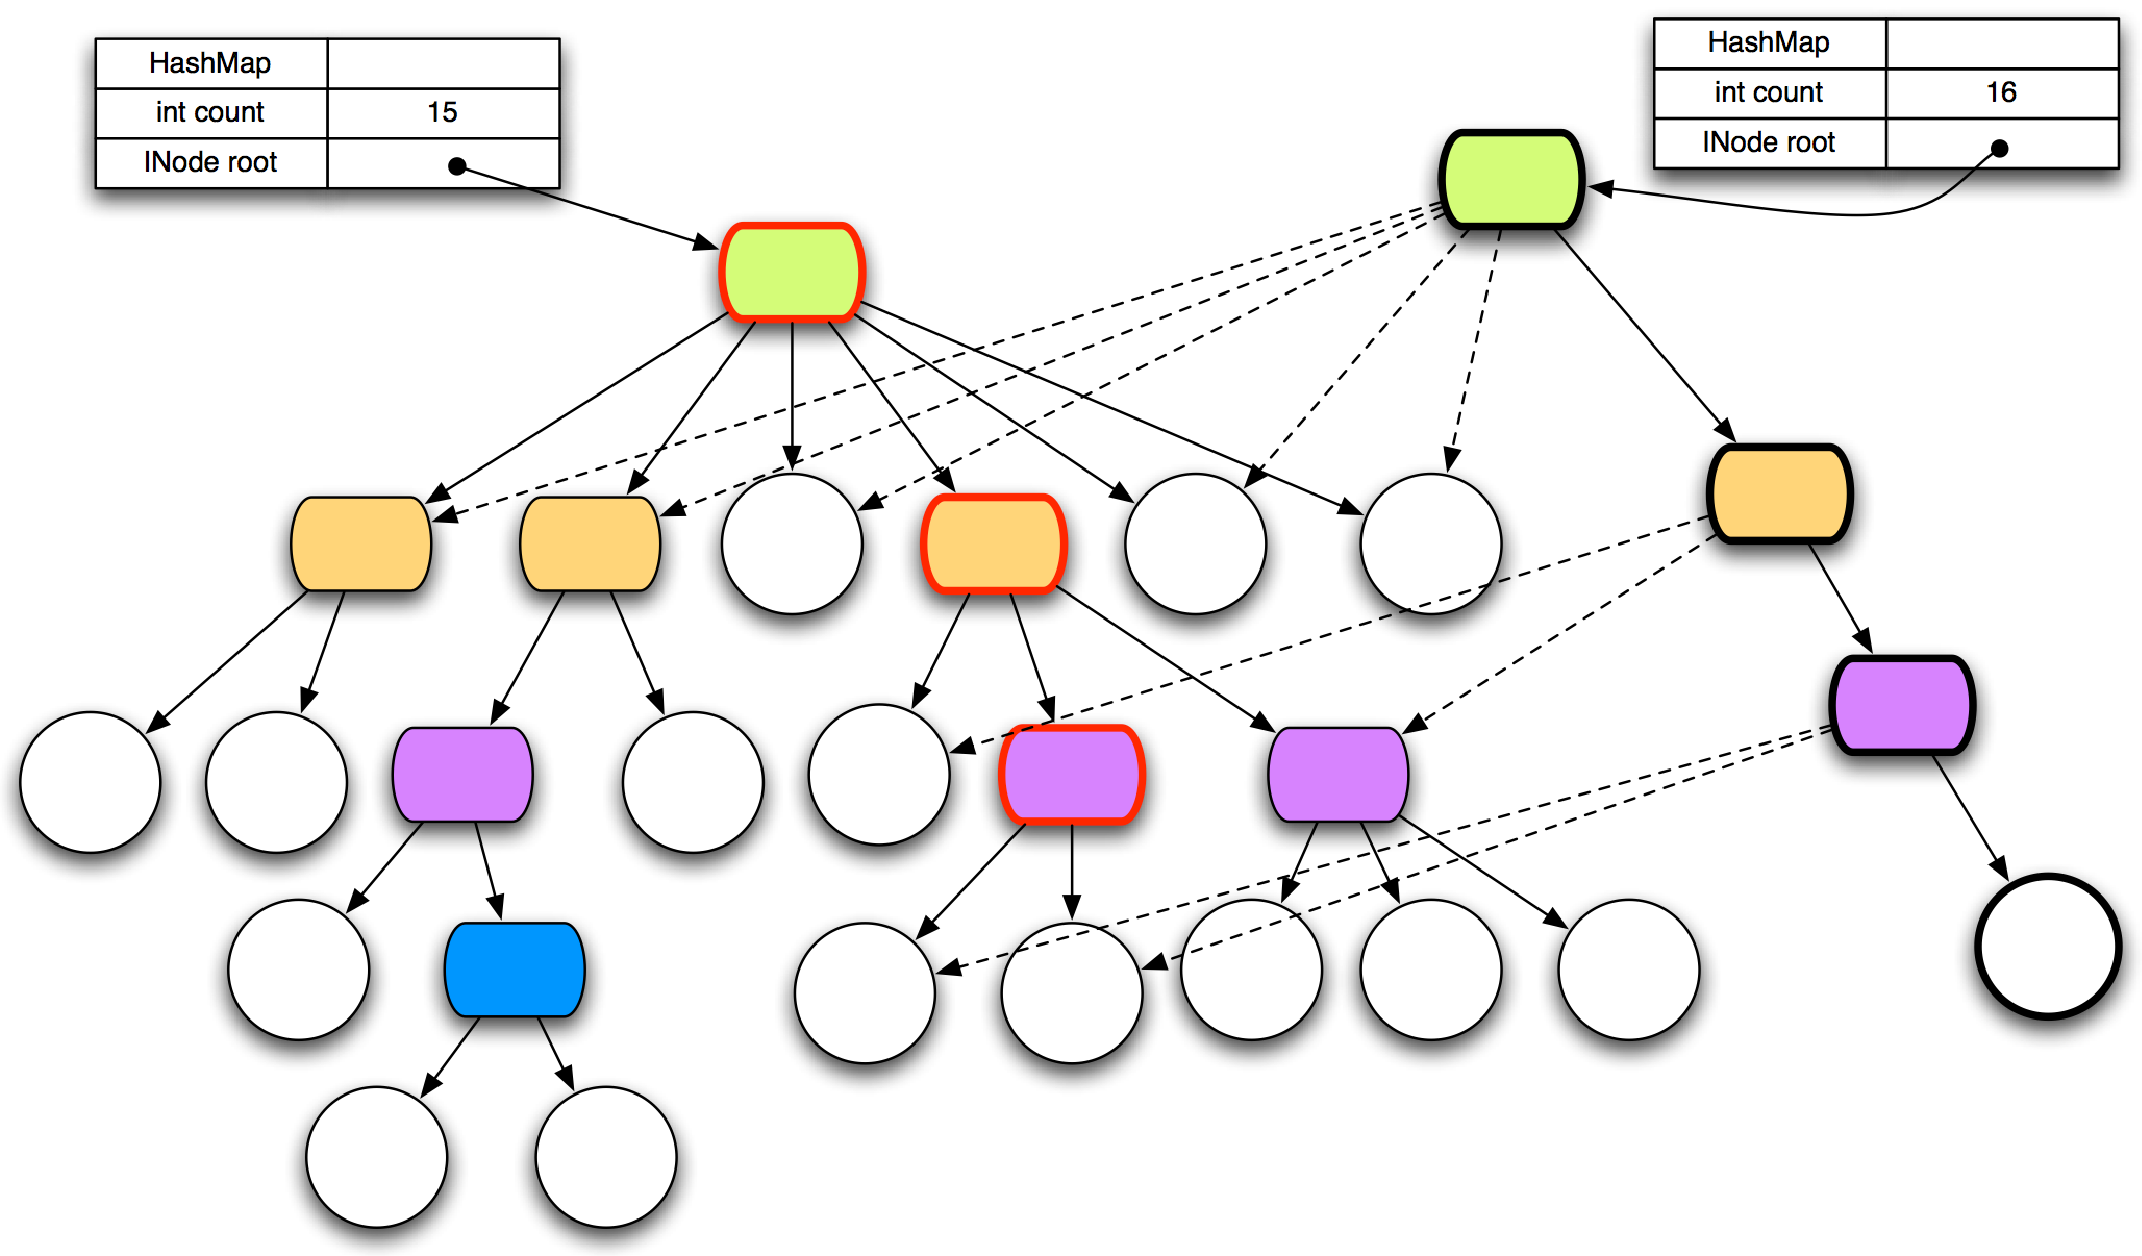
\includegraphics[scale=0.42]{figures/diagrams/persistent-data-structure}
				
				\caption{Representation of how data structures are ``changed'' in Clojure (Source:  \cite{clj-persistent})}
				\label{fig:persistent-data-structure}
			\end{figure}
			
			In \vref{fig:persistent-data-structure}, we see what happens when a persistent data structure is ``changed'' in Clojure.  The root of the left tree is the data structure before, and the root of the right tree is the data structure after.  Note how the changed map retains pointers to all but the updated value; the newly created value is pointed to instead of the previous one.
		
		\subsubsection{Concurrency}
			Clojure supports four systems for concurrency:  \gls{stm}, agents, atoms, and dynamic vars.  The differences between these systems are summarized in \vref{tbl:concurrency-system-comparison}.
			
			\begin{table}
				\centering
				
				\begin{tabular}{llll}
					\toprule
					System Name & Synchronous & Coordinated & Scope \\
					\midrule
					\gls{stm} & Yes & Yes & Application \\
					Agents & No & No & Application \\
					Atoms & Yes & No & Application \\
					Dynamic Vars & Not Applicable & Not Applicable & Thread \\
					\bottomrule
				\end{tabular}
				
				\caption{Comparison between Clojure's four systems for concurrency}
				\label{tbl:concurrency-system-comparison}
			\end{table}
			
			\todo{More concurrency}
			
		\subsubsection{Interoperability With the \gls{jvm}}
			\todo{Compare to other functional languages with decent library support}
			Traditionally, functional programming languages have been undesirable for numerous reasons:  compatibility, libraries, portability, availability, packagability, and tools \cite{no-fp-98}.  Clojure attempts to avoid many of these reasons by running on the \gls{jvm}.  The \gls{jvm} allows Clojure to both call and be called by Java and other languages.  It includes syntactic sugar -- features of a language added in order to simplify the language from a human perspective -- to transparently call Java code, as well as make itself available to Java.  This avoids the above issues.
			
			The syntactic sugar provided by Clojure allows for the accessing of object members, the creation of objects, the calling of methods on an instance or class, etc.  Clojure also includes shortcuts to perform multiple operations on the same object.  The syntax is given in \vref{tbl:jvm-interop-syntax}.
			
			\begin{table}
				\centering
				
				\begin{tabular}{lll}
					\toprule
					Operation & Form & Example \\
					\midrule
					Member Access & \texttt{(.<member> <obj> [args])} & \texttt{(.toString 5)} \\
					 & \texttt{(. <obj> <member> [args])} & \texttt{(. 5 toString)} \\
					 & \texttt{(<class>/<member> [args])} & \texttt{(Integer/parseInt ``5'')} \\
					Object Instantiation & \texttt{(<class>. [args])} & \texttt{(Integer. 5)} \\
					 & \texttt{(new <class> [args])} & \texttt{(new Integer 5)} \\
					Multiple Operations & \texttt{(doto <obj> [forms])} & \texttt{(doto (Vector.) (.add 1))} \\
					\bottomrule
				\end{tabular}
				
				\caption{Syntactic sugar for \gls{jvm} interoperability}
				\label{tbl:jvm-interop-syntax}
			\end{table}
			
			We utilize Clojure's \gls{jvm} interoperability to make use of Apache Lucene and \gls{jdbc}.
			
			\begin{figure}
				\begin{singlespaced}
					\begin{pygments}{clj}
(defn ^Directory idx-path
  [path]
  (-> path File. SimpleFSDirectory.))
					\end{pygments}
				\end{singlespaced}
				
				\caption{Clojure code that, given a path, returns a \texttt{Directory} object}
			\end{figure}
	\section{Search With Clojure}
\label{sec:search-with-clojure}
	Clojure's excellent \gls{jvm} interoperability permits the use of countless third-party libraries.  The most extensively used was Lucene.
	
	\subsection{Full-Text Search Using Lucene}
		\textcquote{luc-home}{Apache Lucene\texttrademark\ is a high-performance, full-featured text search engine library written entirely in Java.}  Lucene implements the Document Model (\cref{sec:document-model}), providing a simple yet powerful \gls{api} to perform full-text search.  Among these features is the ability to vectorize documents according to the Vector Space Model (\cref{sec:vectorization-of-documents}), utilize the extended document model to provide semi-structured documents (\cref{sec:extending-the-document-model}), and issue search queries against the index (\cref{def:search-query}).
	
	\subsection{Indexing Relational Database}
		The indexing of relational objects is a complicated process.  The objects must be retrieved from the relational database, transformed from named tuples into documents, then placed in the index.  Additionally, all foreign keys (\cref{def:foreign-keys}) must be encoded as documents (\cref{sec:encoding-entity-group-as-document-group}) in order to satisfy \cref{sec:mapping-entity-groups-to-documents}.
		
		The schema graph (\cref{def:schema-graph}) must be defined before the relational database may be crawled.
		
		\subsubsection{Schema Graph Definition}
		\label{sec:entity-schema}
			The schema graph is defined using Korma, which \textcquote{clj-korma}{is a \gls{dsl} for Clojure}.  Each schema component, whether an entity or entity group, is defined by \texttt{EntitySchema} records.  Each record accepts a map which specifies how each class of document should be indexed and identified.  The keys of this map are given in \vref{tbl:entity-schema-keys}.
			
			\begin{table}
				\centering
				
				\begin{tabular}{lp{9cm}l}
					\toprule
					Key & Description & Type(s) \\
					\midrule
					\texttt{:T} & Entity (\texttt{:entity}) or entity group (\texttt{:entity}) & Symbol \\
					\texttt{:C} & Table name for entities, brief description for entity groups & Symbol or String \\
					\texttt{:sql} & \Gls{sql} query used to construct the entity or entity schema & Expression \\
					\texttt{:ID} & Attribute or attributes that comprise the key (\vref{def:keys}) & Symbol or list of symbols \\
					\texttt{:attrs} & List of attributes to analyze to fields & List of symbols \\
					\texttt{:values} & List of attributes to index as values, must be subset of \texttt{:attrs} & List of symbols \\
					\bottomrule
				\end{tabular}
				
				\caption{Keys expected by \texttt{EntitySchema} records}
				\label{tbl:entity-schema-keys}
			\end{table}
		
		\subsubsection{Crawling the Relational Database}
			With the schema graph defined, the system is able to crawl the relational database, yielding a sequence of named tuples.  It iterates through every \texttt{EntitySchema} record, instructing every record to crawl itself given a database connection and index writer (\vref{clj:building-the-index}).
			
			\begin{figure}
				\begin{singlespaced}
					\begin{pygments}{clj}
(doseq [ent-def schemas]
  (crawl ent-def db-conn idx-w))
					\end{pygments}
				\end{singlespaced}
				
				\caption{Building the index}
				\label{clj:building-the-index}
			\end{figure}
			
			The \texttt{Database} protocol provides an \texttt{execute-query} method that permits access to the database.  In the current implementation, the \texttt{Sqlite3} record implements the \texttt{Database} protocol.  This record issues the query as-is, applying a given function to every result.
			
			Each record issues a \gls{sql} query against the database that retrieves all named tuples that it represents.  This query is given by the \texttt{:sql} key of the record.  For every symbol defined by the \texttt{:values} key, an additional query is issued.  These queries retrieve all distinct (within the context of that relation and attribute) values.
		
		\subsubsection{Transformation}
			For every named tuple, a document is constructed (see \cref{sec:named-tuples-documents}).  In addition to the attributes, several other fields may be added to the document.  These special fields contain additional meta information about the document.  For example, the class, type, and unique identifier are added to an entity, while an entity group has a space-delimited list of unique identifiers that comprise the group.
			
			Before becoming a document, named tuples are transformed into an internal representation.  The internal representation adds flexibility to the system; so long as functions exist to convert between the internal representation and other forms, the system does not care about the source.
			
			Clojure permits the annotation of data with metadata.  Named tuples are returned as maps, with key-value pairs representing attributes and values for each tuple.  Metadata may be associated with a named tuple that does not affect its key-value pairs.
			
			The map of attributes and values of a named tuple is annotated with the function \texttt{(with-meta obj map)}.  The \texttt{obj} parameter is the named tuple, while \texttt{map} is a map of metadata as defined by the system.  The keys of \texttt{map} for each type (value, entity, or entity group) are defined in \vref{tbl:type-metadata}.
			
			\begin{table}
				\begin{subtable}[b]{0.33\linewidth}
					\centering
					
					\begin{tabular}{ll}
						\toprule
						Key & Value \\
						\midrule
						:type & :value \\
						:class & <rel>|<attr> \\
						\bottomrule
					\end{tabular}
					
					\caption{Value}
				\end{subtable}
				\begin{subtable}[b]{0.33\linewidth}
					\centering
					
					\begin{tabular}{ll}
						\toprule
						Key & Value \\
						\midrule
						:type & :entity \\
						:class & <rel> \\
						:ID & <rel>|<pk> \\
						\bottomrule
					\end{tabular}
					
					\caption{Entity}
				\end{subtable}
				\begin{subtable}[b]{0.33\linewidth}
					\centering
					
					\begin{tabular}{ll}
						\toprule
						Key & Value \\
						\midrule
						:type & :group \\
						:entities & <rel>|<pk> \\
						 & [<rel>|<pk> \ldots] \\
						\bottomrule
					\end{tabular}
					
					\caption{Entity Group}
				\end{subtable}
				
				\caption{Metadata associated with each type}
				\label{tbl:type-metadata}
			\end{table}
			
			The internal representation of the named tuple given in \vref{tbl:hmr-properties} is given in \vref{clj:with-meta-internal-rep}.
			
			\begin{figure}
				\begin{singlespaced}
					\begin{pygments}{clj}
(with-meta
  {:code    "CDPS 101"
   :title   "Human-Mutant Relations"
   :subject "CDPS"}
  {:type  :entity
   :class :course
   :id    "course|cdps_101"})
					\end{pygments}
				\end{singlespaced}
				
				\caption{Internal representation of named tuple from \vref{tbl:hmr-properties}}
				\label{clj:with-meta-internal-rep}
			\end{figure}
			
			Once the internal representation is constructed, it may be transformed into a document.  The mapping of a map to document is trivial; a field is created for every key in the map and the value corresponding to the key is the value of the field.  Unfortunately Lucene does not facilitate the storage of metadata.  Therefore the system must deal with metadata in a different way.
			
			The system modifies each key of the metadata; two underscores are prepended and appended to the key name.  This allows the system to differentiate between metadata and attributes.  The transformation from internal representation to document is given in \vref{tbl:internal-rep-to-document}.
			
			\begin{table}
				\centering
				
				\begin{tabular}{ll}
					\toprule
					Field & Value \\
					\midrule
					code & cdps 101 \\
					title & human mutant relations \\
					subject & cdps \\
					\_\_type\_\_ & entity \\
					\_\_class\_\_ & course \\
					\_\_id\_\_ & course|cdps\_101 \\
					\bottomrule
				\end{tabular}
				
				\caption{Document of internal representation from \vref{clj:with-meta-internal-rep}}
				\label{tbl:internal-rep-to-document}
			\end{table}
		
		\subsubsection{Indexing}
			With the named tuples transformed into documents, the index may be constructed.  The first step is to open the index for writing.  In Lucene, this is accomplished by creating an \texttt{IndexWriter} object on a \texttt{Directory} object that points to the index location.  The \texttt{IndexWriter} object also expects an analyzer to be used by default on documents it indexes.  The system uses a \texttt{WhitespaceAnalyzer} by default.
			
			For every named tuple, the transformed document is written to the index by the index writer object.  In addition, the indexing document (\cref{sec:encoding-entity-group-as-document-group}) of every entity group is added.
		
	\subsection{Keyword Search in Document Space}
	\label{sec:keyword-search-document-space}
		With the entity graph encoded into the document model, users may begin issuing search queries.  Every query follows the following pattern:  users look up values (optionally using fuzzy search), these values are used to locate entities, and once two entities are selected, the system attempts to locate connections between the two.
		
		\subsubsection{Fuzzy Value Search}
			Recall that entity values are stored as their \(n\)-gram (\cref{sec:n-gram}).  This allows users to make character substitutions, deletions, or additions, and still return values they may have intended on finding.  Without the use of \(n\)-grams, a misspelling on the user's part would result in either no or irrelevant values being returned.  Values that are approximately matched would be assigned a lower score than those which are fully matched, but they would at least appear in the results.
			
			Rather than guessing the user's intention, the system presents the user with a list of values in order to give them the option of substituting their entry for an approximate match.  This autosuggest feature is intended to improve the user experience by eliminating a source of frustration -- irrelevant results as a result of a simple spelling error.
		
		\subsubsection{Flexible Keyword Search \gls{api}}
			The system provides a simple -- yet flexible -- keyword search \gls{api}.  Recall the extended query (\cref{ex:extended-query}) is in the form
			\[
				\query(\field, \w)
			\]
			
			The search \gls{api} provides a function that accepts a symbol defining the field to search in, as well one or more words to search for.  A phrase query comprised of every word is constructed.
			\[
				\query(\field, \w_1, \w_2, \dotsc, \w_n) = \bigcap_{\w \in \{\w_1, \w_2, \dotsc, \w_n\}} \query(\field, \w)
			\]
			
			Another function, \texttt{boolean-query}, accepts one or more \(\query\) functions as well as a boolean operator for each and returns the result.  The symbols \texttt{:and}, \texttt{:or}, and \texttt{:not} provide \(\cap\), \(\cup\), and \(\neg\), respectively.
			
			\begin{ex}[\texttt{boolean-query}]
				For example, the query in \cref{ex:extended-query} is given in \vref{clj:boolean-query}.
				
				\begin{figure}
					\begin{singlespaced}
						\begin{pygments}{clj}
(boolean-query
 [[:and (query :subject ``MATH'')]
  [:and (query :text ``class'')]])
						\end{pygments}
					\end{singlespaced}
					
					\caption{Boolean query in Clojure}
					\label{clj:boolean-query}
				\end{figure}
			\end{ex}
		
		\subsubsection{Translation of Search Results to Relational Space}

	\subsection{Graph Search in Document Space}
		With the ability for users to find relevant entities using fuzzy value search and the flexible keyword search \gls{api} (\cref{sec:keyword-search-document-space}), they must be able to find connections between two entities.  As stated previously (\cref{clm:lossless}), the document encoding of relational data is a graph.  This allows the system to search for links between entities by utilizing one or more graph search algorithms, such as \gls{bfs}.
		
		\begin{figure}
			\centering
			
			\begin{dot2tex}[dot]
digraph G {
node [shape=plaintext]; "Human-Mutant Relations"; "Community Development & Policy Studies";

"Human-Mutant Relations" -> "Community Development & Policy Studies";
}
			\end{dot2tex}
			
			\caption{Human-Mutant Relations entity group}
			\label{fig:hmr-entity-group}
		\end{figure}
		
		\subsubsection{Why We Need Graph Search}
			Tuples are fragments, or facts, of larger pieces of knowledge.  By utilizing graph search, we amalgamate these facts to provide a user with a broader view.
			
			\begin{ex}
				By utilizing graph search, we can take the facts in \cref{tbl:facts} and compose new facts.  For example, we could learn who teaches Complex Analysis.  It also allows us to ask questions, such as ``who taught Complex Analysis with Instructor X?''
				
				\begin{table}
					\begin{subtable}[b]{0.5\linewidth}
						\centering
						
						\begin{tabular}{ll}
							\toprule
							Field & Terms \\
							\midrule
							code & \(\{\text{math}, \text{360}\}\) \\
							title & \(\{\text{complex}, \text{analysis}\}\) \\
							subject & \(\{\text{math}\}\) \\
							\bottomrule
						\end{tabular}
						
						\caption{Fact representing a Course}
						\label{subtbl:fact-course}
					\end{subtable}
					\begin{subtable}[b]{0.5\linewidth}
						\centering
						
						\begin{tabular}{ll}
							\toprule
							Field & Terms \\
							\midrule
							id & \(\{\text{math}\}\) \\
							name & \(\{\text{mathematics}\}\) \\
							\bottomrule
						\end{tabular}
						
						\caption{Fact representing a Subject}
						\label{subtbl:fact-subject}
					\end{subtable}
					
					\caption{Fragments, or facts, of information in a dataset}
					\label{tbl:facts}
				\end{table}
			\end{ex}
			
			This automated discovery of relations between facts is why graph search is important.
		
		\subsubsection{Graph Search Algorithms}
			Recall we defined a graph as \(G = (V, E)\), where \(V\) is the set of all facts in the database, and \(E\) is the set of relations between facts.
		
		\subsubsection{Graph Search in Document Space}
			
		
		Graph search algorithms
		=======================
		
		%# Definition of the graph
		
		G = (V, E)
		
		V = all entity-groups in DB
		Let $Ent(v)$ be the set of entities in entity group $v$.
		We say that two vertices in $G$ are connected if and only if:
		
		$Ent(v)\cap Ent(v')\not=\emptyset$.
		
		%# Definition of graph search
		
		Given a keyword query q, find a subgraph, $H$, of G to:
		- minimize the vertices in H
		- maximize the satisfaction of keywords in $q$ by vertices in $H$.
		
		Example (based on UOIT or superhero) should be given here.
		- just use the canonical example for benchmark testing.
		
		%# Logical specification of the graph search algorithm:
		
		- find all vertices by entity group search, and call this C.
		- use any graph search algorithm to minimally connect the vertices in C
		as follows. 
		let s\in C be a source.
		for each t\in C-{s}:
		find path connecting s->t such that len(path) <= user-defined-bound.
		
		%# Why use document space for graph search (THESIS OF YOUR THESIS)
		
		- finding the relevant "seed" vertices is really fast.  This is done by
		using full text search on the documents of an entity graph.  Therefore, it
		allows fuzzy search for the seeds.
		- finding connected entity groups is really fast - this is done by using the
		indexing document.  Using a single keyword query, we can find all relevant
		entity groups in the database.
		
		Example: spell this out:
		
		index-doc(v0) = student:ABC, course:XYZ
		query: (:or (:and (id:ABC) (C:student)) 
		(:and (id:XYZ) (C:course)))
		
		%# Breadth-first search
		
		Description: copy this from CLRS
		<Richard>
		
		Functional description of BFS
		
		Distributed functional description of BFS
		
		Implementation details:
		- Ref
		- Atoms
		- Agent
		
		\begin{itemize}
			\item Why we need graph search
			\item Search in document graph using graph search algorithms with functional implementations: (Ford Fulkerson, BFS)
			\item Speed up using concurrency
			\item Clojure specific optimization: ref + atom
		\end{itemize}
	
	\chapter{Experimental Evaluation}
\label{chap:experimental-evaluation}
	In this chapter we evaluate our implementation of the system for transforming data in the relational model to the document model and vice versa described in \cref{chap:tale-of-two-data-models}.  We cover the implementation details in \cref{sec:implementation}, and the methodology and evaluation in \cref{sec:runtime-evaluation}.
	
	\section{Implementation}
	\label{sec:implementation}
		The system was implemented in Clojure, which \textcquote{clj-home}{is a dynamic programming language that targets the \gls{jvm}}.  Clojure was chosen due to its rich, immutable, and persistent data structures, first-class concurrency support, and seamless \gls{jvm} interoperability.  These features were discussed in detail in \cref{sec:features-of-clojure}.
		
		\subsection{Code Base Statistics}
			The system consists of over 800 lines of Clojure, along with approximately 550 lines of Python.  The Python code is used to construct the data set by crawling the course information site, as well as to aggregate the benchmark data produced by the system, producing graphs.
			
			All development has occurred on GitHub \cite{molly-repo}.  The use of Git and GitHub permits collaboration between researchers.  With the code publicly available, future researchers may study, run, and, build upon it.
	
	\section{The Data Corpus}
	\label{sec:data-corpus}
		The data corpus was derived from the \gls{uoit} mycampus database.  It is not a standard dataset used in the literature, but a dataset unique to \gls{uoit}.
		
		An \gls{html} crawler was written in Python that scraped the information from the \gls{uoit} class schedule search page.  This data was parsed, normalized, then placed in a SQLite database.
		
		The data corpus consists of numerous classes of objects.  These are:  courses (\cref{tbl:corpus-course}), instructors (\cref{tbl:corpus-instructor}), schedules (\cref{tbl:corpus-schedule}), sections (\cref{tbl:corpus-section}), and teaches (\cref{tbl:corpus-teaches}).  A graph representation of how these classes of objects are related can be found in \cref{fig:schema-graph}.  The data corpus is defined in \cref{chap:data-corpus-def}
		
		The number of objects, as of the publication of this thesis, can be found in \cref{tbl:data-corpus-count}.
		
		\begin{table}
			\centering
			\begin{tabular}{lr}
			\toprule
			Class & Count \\
			\midrule
			Course & 1340 \\
			Instructor & 849 \\
			Schedule & 25755 \\
			Section & 14463 \\
			Teaches & 15358 \\
			\bottomrule
			\end{tabular}
			
			\caption{Number of objects in data corpus, grouped by class}
			\label{tbl:data-corpus-count}
		\end{table}
	
	\section{Runtime Evaluation}
	\label{sec:runtime-evaluation}
		Scripts were written to coordinate the execution, collection, and transformation of the performance data of our implementation.
		
		\subsection{Methodology}
			We used Criterium\footnote{\url{http://hugoduncan.org/criterium/}} to handle the execution of the benchmarks as it handles unique concerns stemming from benchmarking on the \gls{jvm}.  These issues, identified by \citeauthor{rob-java-bench-08} \cite{rob-java-bench-08}, include:
			
			\begin{itemize}
				\item Statistical processing of multiple evaluations
				\item Inclusion of a warm-up period which is intended to allow the JIT compiler to translate the Java byte code into native instructions
				\item Purging of the garbage collector before testing, to isolate timings from GC state prior to testing
				\item A final forced garbage collection after testing to estimate impact of cleanup on the timing results
			\end{itemize}
			
			As each function is invoked numerous times, this greatly increases the runtime.
			
			During evaluation, Criterium collects performance metrics.  Upon completion of the evaluation, it performs statistical analysis of these metrics using the bootstrap procedure developed by \citeauthor{efron-87} \cite{efron-87}.  These metrics include mean, samples, variance, quartiles, outliers, and more.
		
			\subsubsection{Data Collection}
			\label{sec:data-collection}
				The performance metrics computed by Criterium are returned as a Clojure map data structure.  The evaluation process may take several hours to complete, necessitating a separation between data collection and post-processing.  These metrics are stored offline for further processing.
				
				A data interchange format (\gls{json}) is used to utilize the Clojure output in Python.  The benchmark function writes the Criterium performance analysis out as a \gls{json} string to stdout and the output is captured by the benchmark script.  An example of this \gls{json} output is given in \cref{fig:criterium-json-output}.
				
				\begin{figure}
					\centering % Pointless, but who knows in the future.
					\begin{verbatim}
                    [{
                        "max-hops": ...,
                        "method": ...,
                        "results": {
                            "execution-count": ...,
                            "final-gc-time": ...,
                            "lower-q": [...],
                            "mean": [...],
                        ...
                    }, ...]
					\end{verbatim}
					
					\caption{Partial \gls{json} output from Criterium.}
					\label{fig:criterium-json-output}
				\end{figure}
		
		\subsection{Performance}
		\label{sec:performance}
			Performance was measured for the system components.  An analysis of the metrics collected is presented in this section.
			
			\subsubsection{Indexing}
				The indexing process is computationally intensive but short lived.  After the initial \gls{jvm} warmup period, the time required to construct the index scales with the number of named tuples and relations between them.
				
				\begin{table}
					\centering
					\begin{tabular}{ll}
						\toprule
						Number of Groups & Elapsed Time (s) \\
						\midrule
						0 & 11.800 \\
						1 & 12.446 \\
						2 & 19.771 \\
						\bottomrule
					\end{tabular}
					
					\caption{Indexing time growth by number of entity groups, averaged over 5 runs}
					\label{tbl:index-growth-entity-groups}
				\end{table}
				
				We see in \cref{tbl:index-growth-entity-groups} the indexing time increases minimally between 0 and 1 group.  Few entity groups are created by the first entity schema.  Contrast this to the indexing time between 1 and 2 groups, which increases considerably.  The number of entity groups also grew considerably, explaining the time increase.
			
			\subsubsection{Graph Search}
				The worst-case performance of \gls{bfs} is \(\mathcal{O}(n^2)\).  This is reflected in \cref{fig:growth} which follows an exponential growth curve.  In an attempt to mitigate the rapid increase in search time, concurrent variants of \gls{bfs} were also implemented and benchmarked.
				
				\begin{figure}
					\centering
					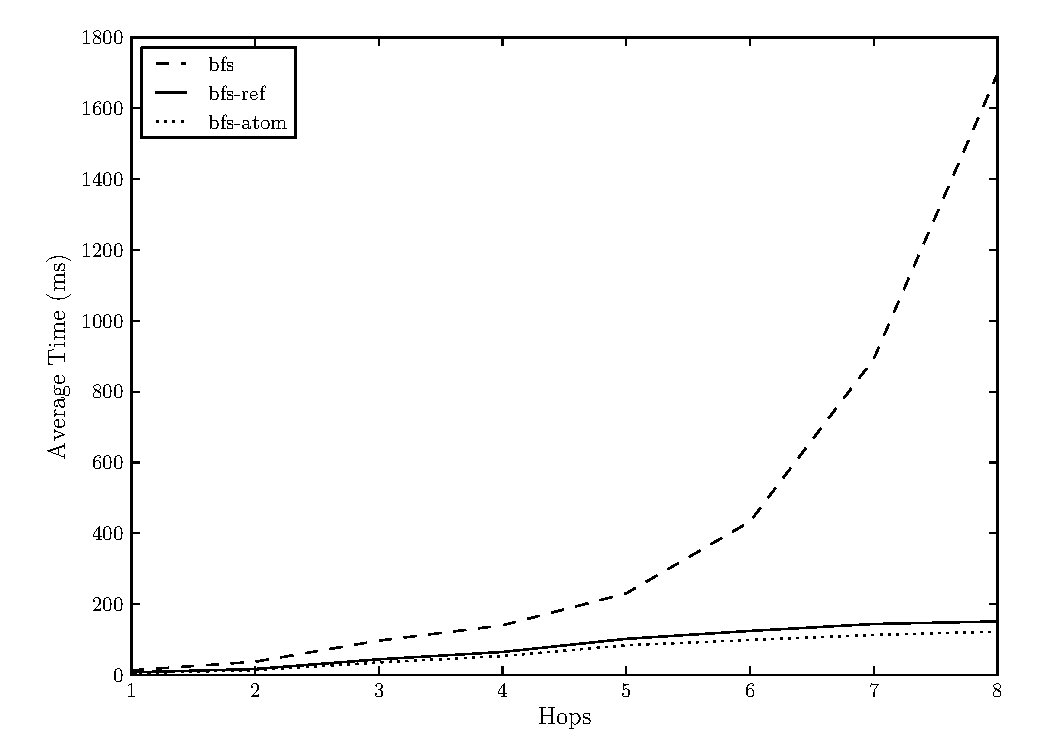
\includegraphics[scale=0.9]{figures/charts/growth.pdf}
					\caption{Growth of each graph search algorithm implementation by number of hops}
					\label{fig:growth}
				\end{figure}
				
				We see in \cref{fig:growth} the rate of growth of \gls{bfs} is as expected.  The rate of growth of \gls{bfs} with references and \gls{bfs} with atoms is nearly linear.  The atom implementation is slightly more performant as it lacks some of the overhead associated with references.
				
				\begin{figure}
					\begin{subfigure}[b]{.5\linewidth}
						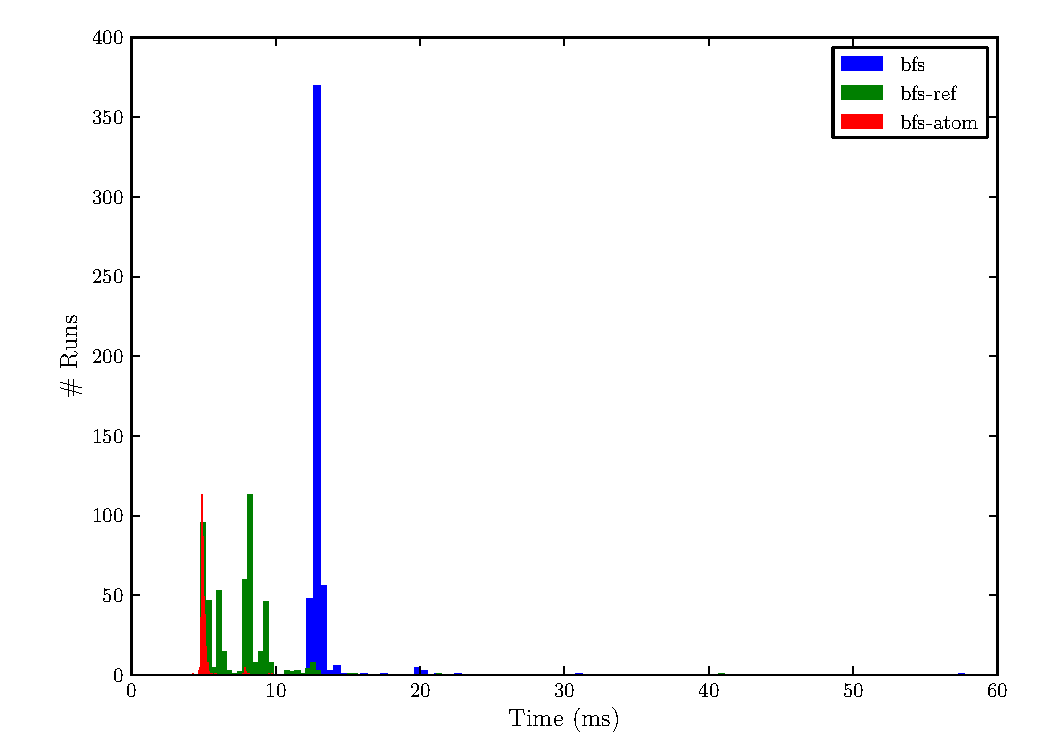
\includegraphics[scale=0.45]{figures/charts/1_hops.pdf}
						\caption{1 Hop}
						\label{subfig:1-hop}
					\end{subfigure}
					\begin{subfigure}[b]{.5\linewidth}
						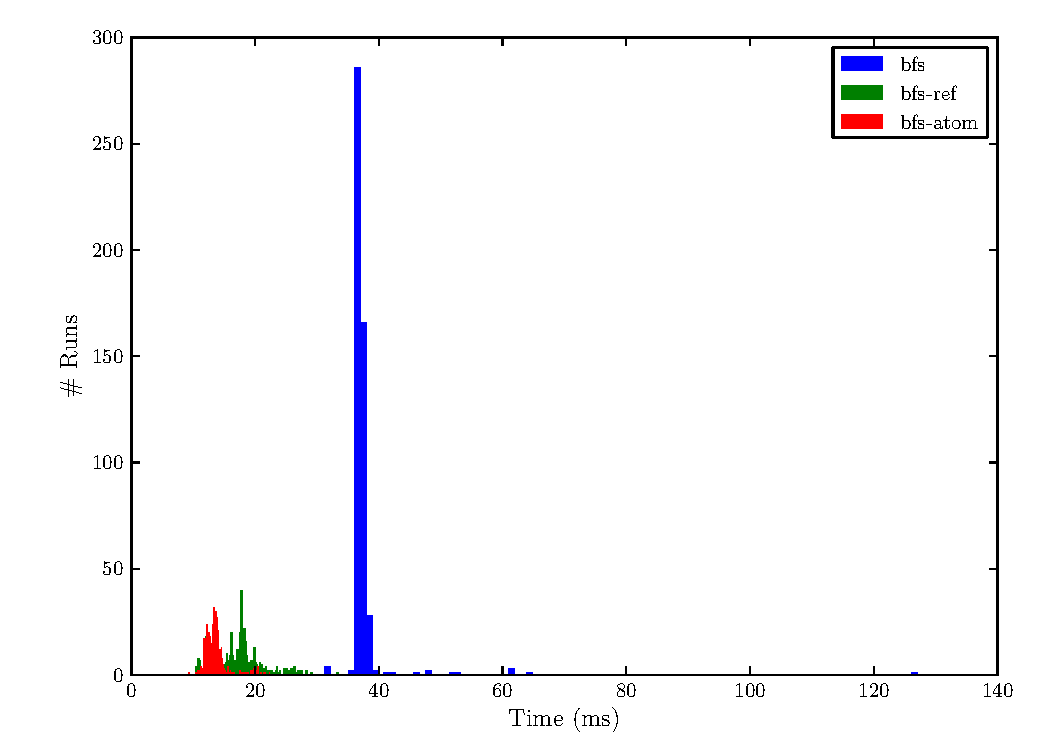
\includegraphics[scale=0.45]{figures/charts/2_hops.pdf}
						\caption{2 Hops}
						\label{subfig:2-hops}
					\end{subfigure}
				\end{figure}
				\begin{figure}
					\ContinuedFloat
					\begin{subfigure}[b]{.5\linewidth}
						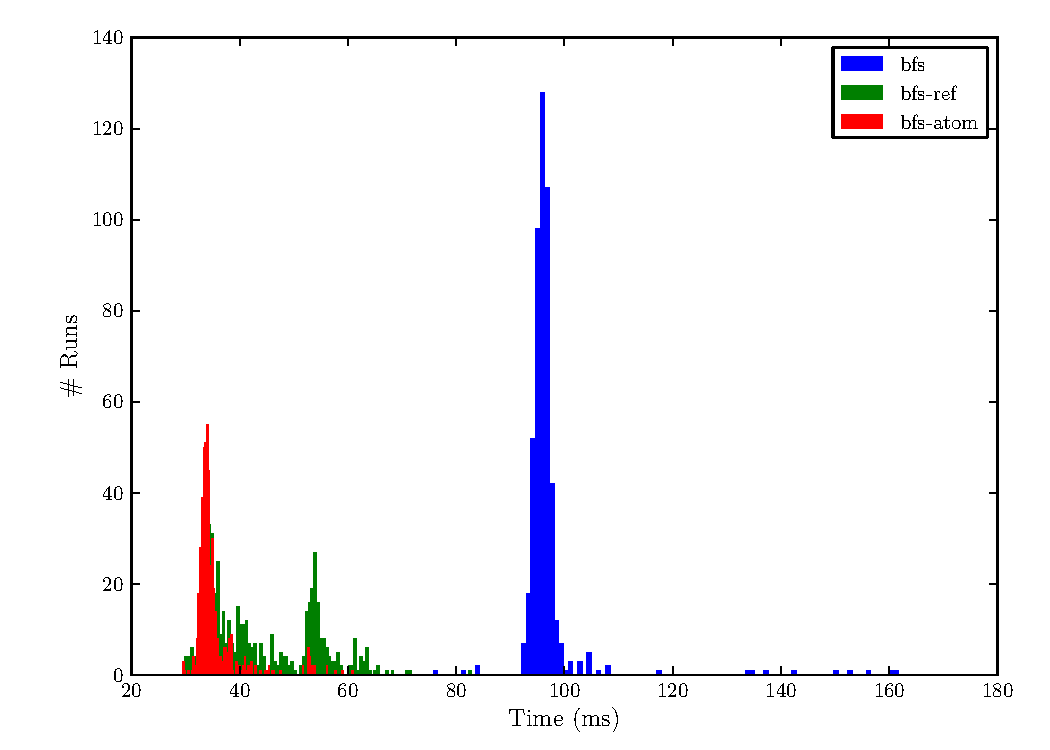
\includegraphics[scale=0.45]{figures/charts/3_hops.pdf}
						\caption{3 Hops}
						\label{subfig:3-hops}
					\end{subfigure}
					\begin{subfigure}[b]{.5\linewidth}
						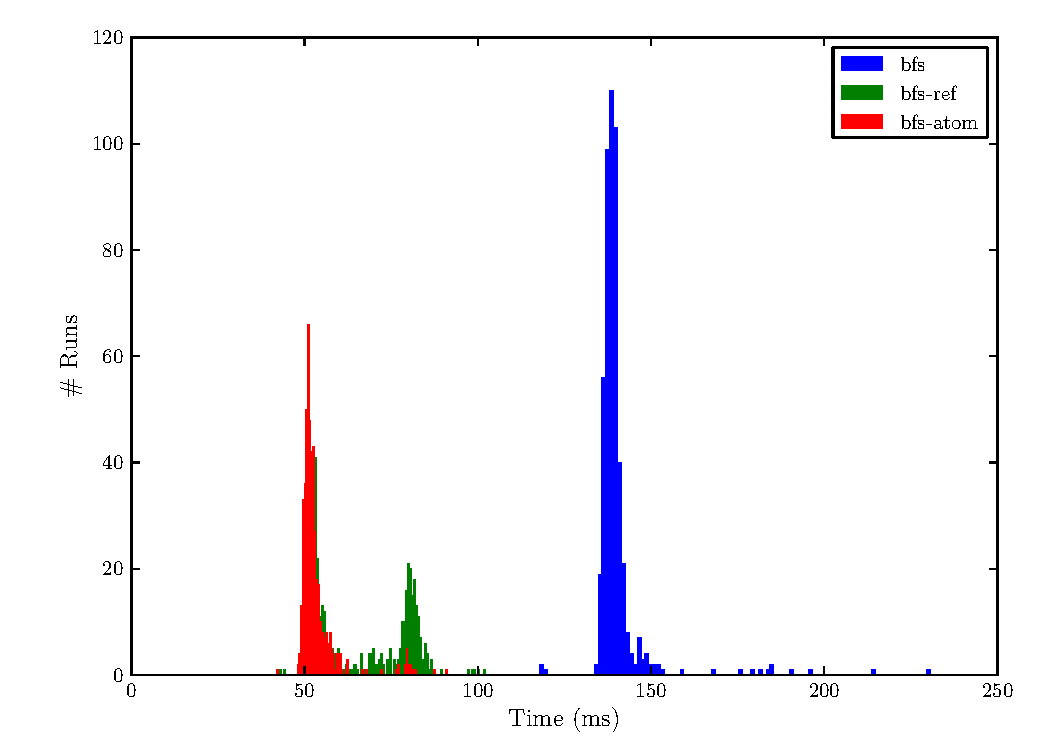
\includegraphics[scale=0.45]{figures/charts/4_hops.pdf}
						\caption{4 Hops}
						\label{subfig:4-hops}
					\end{subfigure}
				\end{figure}
				
				\begin{figure}
					\ContinuedFloat
					\begin{subfigure}[b]{.5\linewidth}
						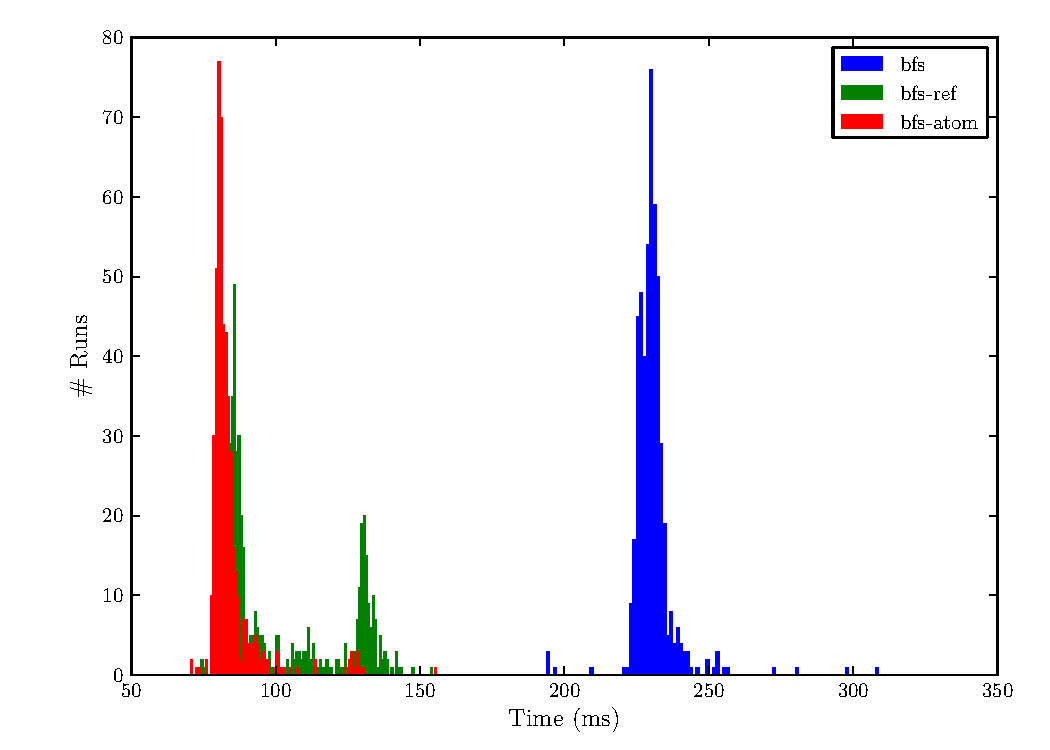
\includegraphics[scale=0.45]{figures/charts/5_hops.pdf}
						\caption{5 Hops}
						\label{subfig:5-hops}
					\end{subfigure}
					\begin{subfigure}[b]{.5\linewidth}
						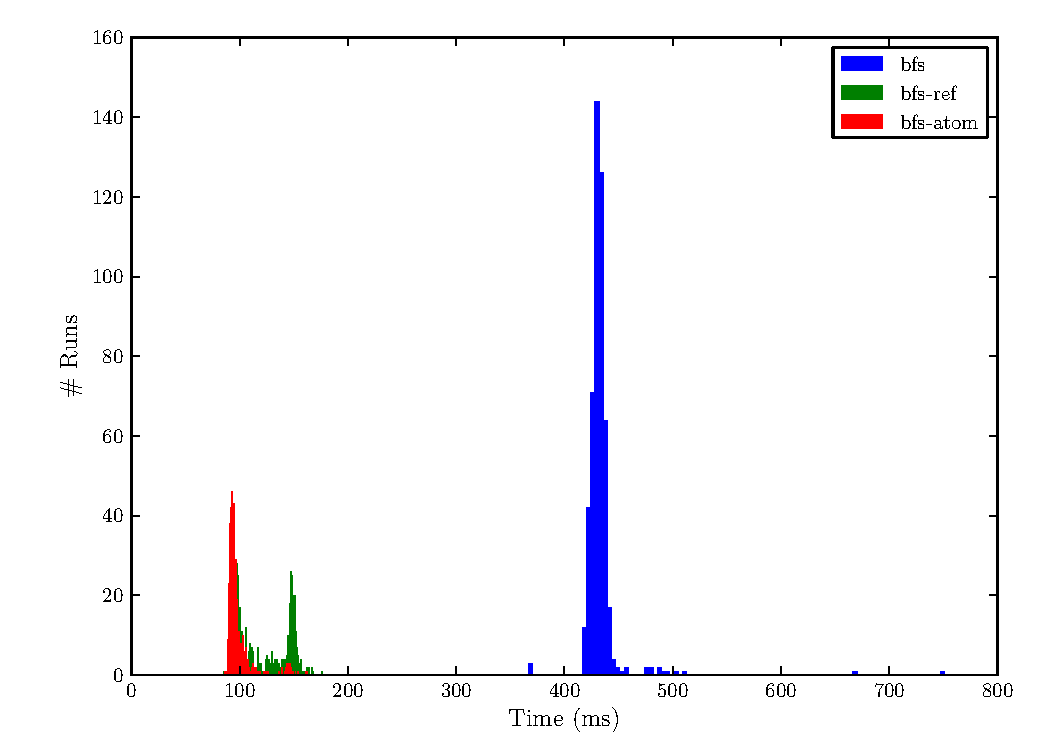
\includegraphics[scale=0.45]{figures/charts/6_hops.pdf}
						\caption{6 Hops}
						\label{subfig:6-hops}
					\end{subfigure}
				\end{figure}
				\begin{figure}
					\ContinuedFloat
					\begin{subfigure}[b]{.5\linewidth}
						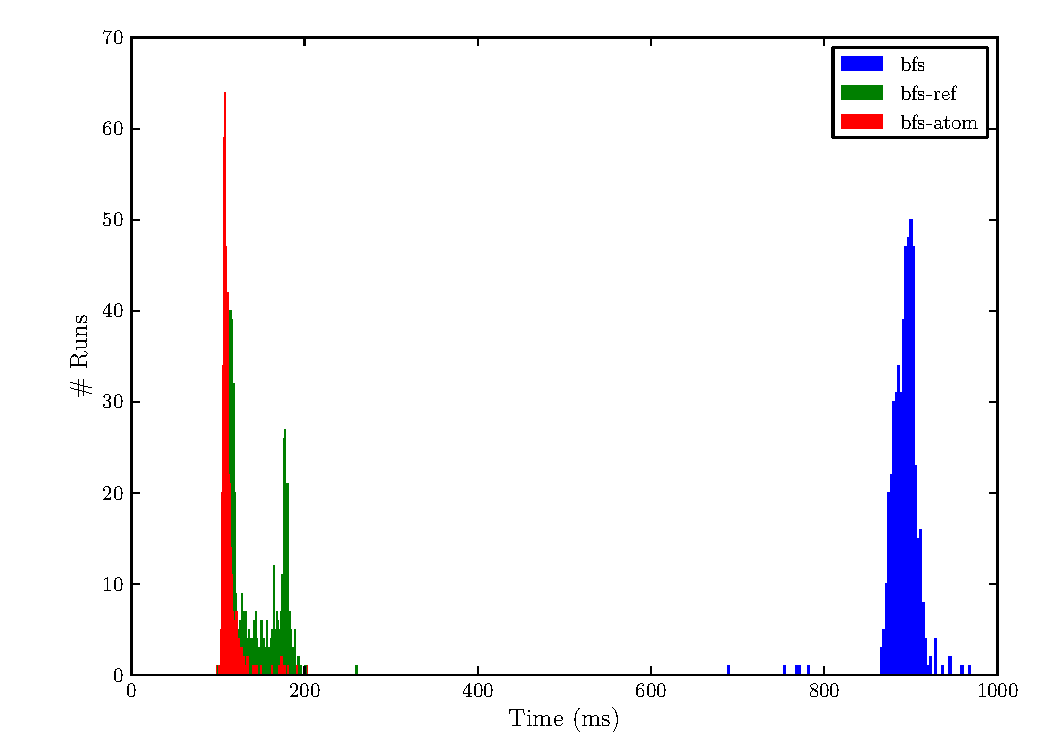
\includegraphics[scale=0.45]{figures/charts/7_hops.pdf}
						\caption{7 Hops}
						\label{subfig:7-hops}
					\end{subfigure}
					\begin{subfigure}[b]{.5\linewidth}
						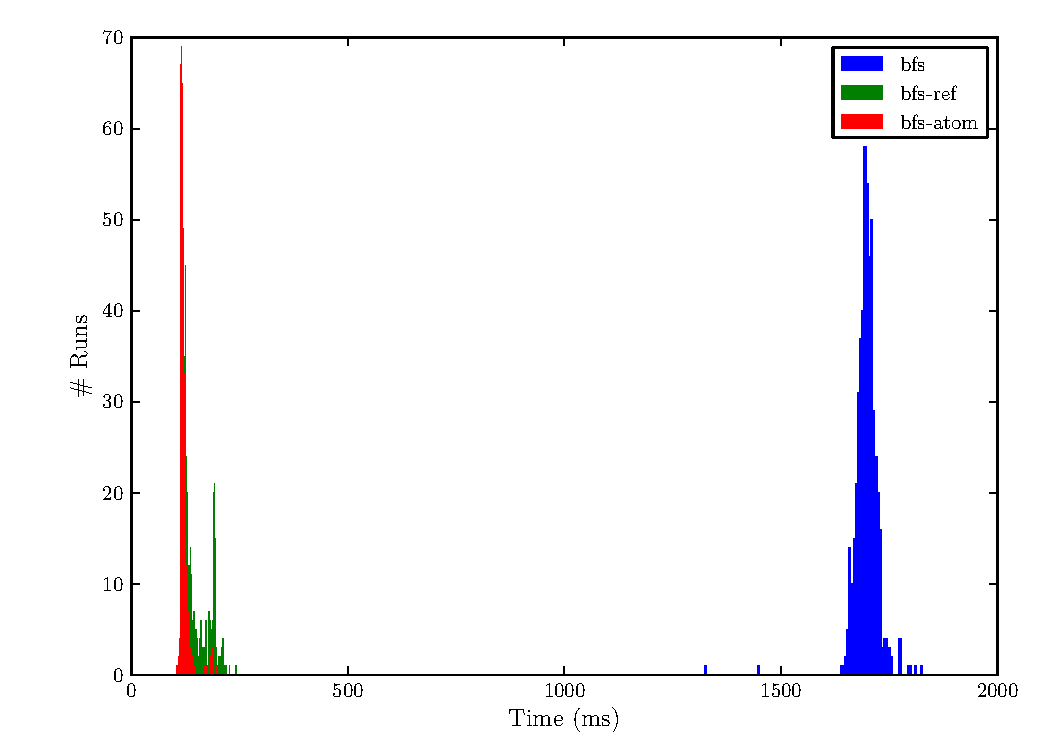
\includegraphics[scale=0.45]{figures/charts/8_hops.pdf}
						\caption{8 Hops}
						\label{subfig:8-hops}
					\end{subfigure}
					
					\caption{Distribution of samples per method, broken down by hops}
					\label{fig:distribution-hops}
				\end{figure}
				
				The difference in rate of growth is further illustrated in \cref{fig:distribution-hops}.  As seen previously, \cref{subfig:1-hop} shows little difference in runtime between the three methods.  The difference becomes clearer in \cref{subfig:2-hops}, and by \cref{subfig:8-hops}, the difference is obvious.
				
				By using a profiling tool\footnote{\url{http://yourkit.com/}}, we see the behaviour of Clojure's concurrency implementation.
				
				\begin{figure}
					\centering
					
					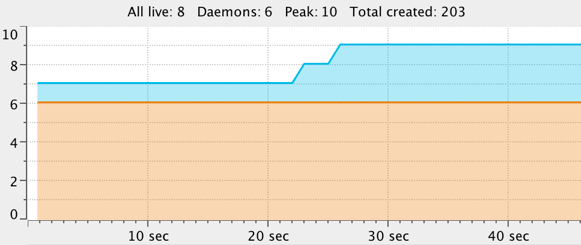
\includegraphics{figures/images/threads}
					
					\caption{Thread count while running \gls{bfs} atom benchmark}
					\label{fig:runtime-threads}
				\end{figure}
				
				In \cref{fig:runtime-threads} we see that a number of threads are created and destroyed.  Recall a new thread is created every time the frontier is populated.
	
	\section{Threats to Validity}
	\label{sec:threats-to-validity}
		No experiment is without its flaws.  In this section we discuss the factors that may affect the validity of the experimental evaluation.  These factors are referred to as threats to validity.  These threats are categorized as internal, external, construct, and conclusion.
		
		\subsection{Internal Validity}
		\label{sec:internal-validity}
			\begin{displayquote}[\cite{wohlin-10}]
				If a relationship is observed between the treatment and the outcome, we must make sure that it is a causal relationship, and that it is not a result of a factor of which we have no control or have not measured. In other words that the treatment causes the outcome (the effect).
			\end{displayquote}
		
		\subsection{External Validity}
		\label{sec:external-validity}
			\begin{displayquote}[\cite{wohlin-10}]
				The external validity is concerned with generalization.
			\end{displayquote}
			
			We used a non-standard dataset to evaluate the system.  This dataset was originally chosen due to its reasonable size.  It also originated from a relational database.  A standard dataset, such as DBLP\footnote{\url{http://dblp.uni-trier.de/}}, is semi-structured and thus unsuitable to demonstrate the transformation from relational data.  The choice of a non-standard dataset makes it difficult to compare performance across systems.
			
			The use of a single dataset presents another issue.  By only using one dataset, it is difficult to generalize the results.  Ideally multiple datasets, each with varying characteristics, would have been used for evaluation.  This is potential area for future work to be done.
		
		\subsection{Construct Validity}
		\label{sec:construct-validity}
			\begin{displayquote}[\cite{wohlin-10}]
				This validity is concerned with the relation between theory and observation.
			\end{displayquote}
		
		\subsection{Conclusion Validity}
		\label{sec:conclusion-validity}
			\begin{displayquote}[\cite{wohlin-10}]
				This validity is concerned with the relationship between the treatment and the outcome.
			\end{displayquote}
	
	\section{Summary}
	\label{sec:eval-summary}
		The system was implemented primarily in Clojure with supporting code written in Python.  The Python code was used to produce the mycampus dataset which was used in the evaluation.  It was also used to orchestrate the execution of benchmarks.
		
		In \cref{sec:runtime-evaluation} we described the experimental methodology and data collection.  We then evaluated the performance of the system using said methodology.  The results demonstrated that the growth of \gls{bfs} can be mitigated by the use of concurrency.  Clojure facilitated a natural transition from a classical implementation of \gls{bfs} to a highly concurrent one.
		
		The assessment of system performance was not without its flaws.  These were discussed in \cref{sec:threats-to-validity}.  The primary threat to validity was the lack of comparison between other systems and datasets.  It is difficult to generalize the results as a result.
		
		Benchmarking any code is difficult.  The process may not have exclusive control over the processor, memory is paged in and out, disk I/O is cached, etc.  The \gls{jvm} complicates matters with \gls{jit} compilation and garbage collection.
	
	\chapter{Conclusion (0 days)}
		Survived Clojure.

	\appendix
	
	\begin{singlespaced}
		% !TEX root = Thesis.tex
	
\chapter{Source Code}
	Each namespace in the code is divided into sections in the thesis document.
	  
	\section{molly}
		\subsection{molly.core}
			The core namespace is responsible for determining, provided a series of command line arguments, which action to take.  This namespace is invoked as the main class when the \gls{jar} is executed.
			
			\inputpygments{clj}{../../src/clj/molly/core.clj}
	
	\clearpage
	\section{molly.conf}
		\subsection{molly.conf.config}
			This namespace contains helper functions for loading part of the system configuration.  It also provides a protocol, \texttt{IConfig}, that is used to define the rest of the system configuration.
			
			\inputpygments{clj}{../../src/clj/molly/conf/config.clj}
		  
		\clearpage
		\subsection{molly.conf.mycampus}
			This is a sample configuration.  It defines the entities and relations in the mycampus dataset.
			
			\inputpygments{clj}{../../src/clj/molly/conf/mycampus.clj}
	
	\clearpage
	\section{molly.datatypes}
		There are several datatypes used in the system.
		\subsection{molly.datatypes.database}
			A protocol and concrete datatype are defined which provide access to a relational database.  Users creating an instance of this datatype are able to execute arbitrary queries, and must provide a function to apply to every tuple that is returned.
			
			\inputpygments{clj}{../../src/clj/molly/datatypes/database.clj}
		
		\clearpage
		\subsection{molly.datatypes.entity}
			One of the most important namespaces represents entities.  It includes functions to transform a named tuple from a database row into the internal representation as well as into documents.  It also includes auxiliary functions to produce a unique identifier.
			
			\inputpygments{clj}{../../src/clj/molly/datatypes/entity.clj}
		
		\clearpage
		\subsection{molly.datatypes.schema}
			The final datatype represents a schema.  These schemas contain a function that is used to execute the necessary \gls{sql} statements to retrieve all data from the relational database and place it in the full-text search index.
			
			Several of these schema datatypes are joined together in a configuration to produce a schema graph.
			
			\inputpygments{clj}{../../src/clj/molly/datatypes/schema.clj}
	
	\clearpage
	\section{molly.index}
		\subsection{molly.index.build}
			This namespace contains the function used to build the full-text search database.  It takes advantage of the fact that each schema knows how to construct its own documents.  The function simply iterates through every schema in the configuration, instructing them to index themselves.
			
			\inputpygments{clj}{../../src/clj/molly/index/build.clj}
	
	\clearpage
	\section{molly.util}
		\subsection{molly.util.nlp}
			The \texttt{q-gram} function computes the \(q\)-gram of a string.  Optionally a value for \(q\) and the padding character can be specified.
			
			\inputpygments{clj}{../../src/clj/molly/util/nlp.clj}
	
	\clearpage
	\section{molly.search}
		\subsection{molly.search.lucene}
			This namespace contains functions for interfacing with the Lucene library.  These functions include opening, adding documents, searching, and closing indices.
			
			\inputpygments{clj}{../../src/clj/molly/search/lucene.clj}
		
		\clearpage
		\subsection{molly.search.query\_builder}
			Phrase queries are used as they require each term in the phrase to be in a specific order.  This permits more accurate results as course titles and other items are in a specific order.
			
			These queries may be combined, creating a boolean query.
			
			\inputpygments{clj}{../../src/clj/molly/search/query_builder.clj}
	
	\clearpage
	\section{molly.server}
		This namespace contains functionality to expose the system functionality to clients over \gls{http}.
		
		\subsection{molly.server.core}
			\inputpygments{clj}{../../src/clj/molly/server/core.clj}
		
		\clearpage
		\subsection{molly.server.remotes}
			Rather than handle serialization over \gls{http} manually, the system uses the Shoreleave library\footnote{\url{https://github.com/shoreleave/shoreleave-remote}}.  It permits ClojureScript clients to transparently call functions exposed on the server.  The \texttt{defremote} macro is used to expose these functions.
			
			\inputpygments{clj}{../../src/clj/molly/server/remotes.clj}
		
		\clearpage
		\subsection{molly.server.search}
			This namespace provides the ``glue'' between the system and \gls{http} interface.
			
			\inputpygments{clj}{../../src/clj/molly/server/search.clj}
	
	\clearpage
	\section{molly.algo}
		\subsection{molly.algo.common}
			\inputpygments{clj}{../../src/clj/molly/algo/common.clj}
		
		\clearpage
		\subsection{molly.algo.bfs}
			\inputpygments{clj}{../../src/clj/molly/algo/bfs.clj}
		
		\clearpage
		\subsection{molly.algo.bfs\_atom}
			\inputpygments{clj}{../../src/clj/molly/algo/bfs_atom.clj}
		
		\clearpage
		\subsection{molly.algo.bfs\_ref}
			\inputpygments{clj}{../../src/clj/molly/algo/bfs_ref.clj}
	
	\clearpage
	\section{molly.bench}
		\subsection{molly.bench.benchmark}
			\inputpygments{clj}{../../src/clj/molly/bench/benchmark.clj}
	\end{singlespaced}
	
	\printbibliography
	
	\todos
\end{document}
s
